\documentclass{oblivoir}

\usepackage{graphicx, jiwonlipsum, subfig}
\graphicspath{{./pictures/}{./pictures01}}

\usepackage{tabu}
\usepackage{xcolor, multirow}
\definecolor{Plum}{rgb}{0.56, 0.27, 0.52}
\definecolor{OliveDrab}{rgb}{0.42, 0.56, 0.14}
\definecolor{RedViolet}{rgb}{0.78, 0.08, 0.52}
\definecolor{Brown}{rgb}{0.65, 0.16, 0.16}
\definecolor{Blue}{rgb}{0, 0, 1}

\begin{document}

%\begin{center}
%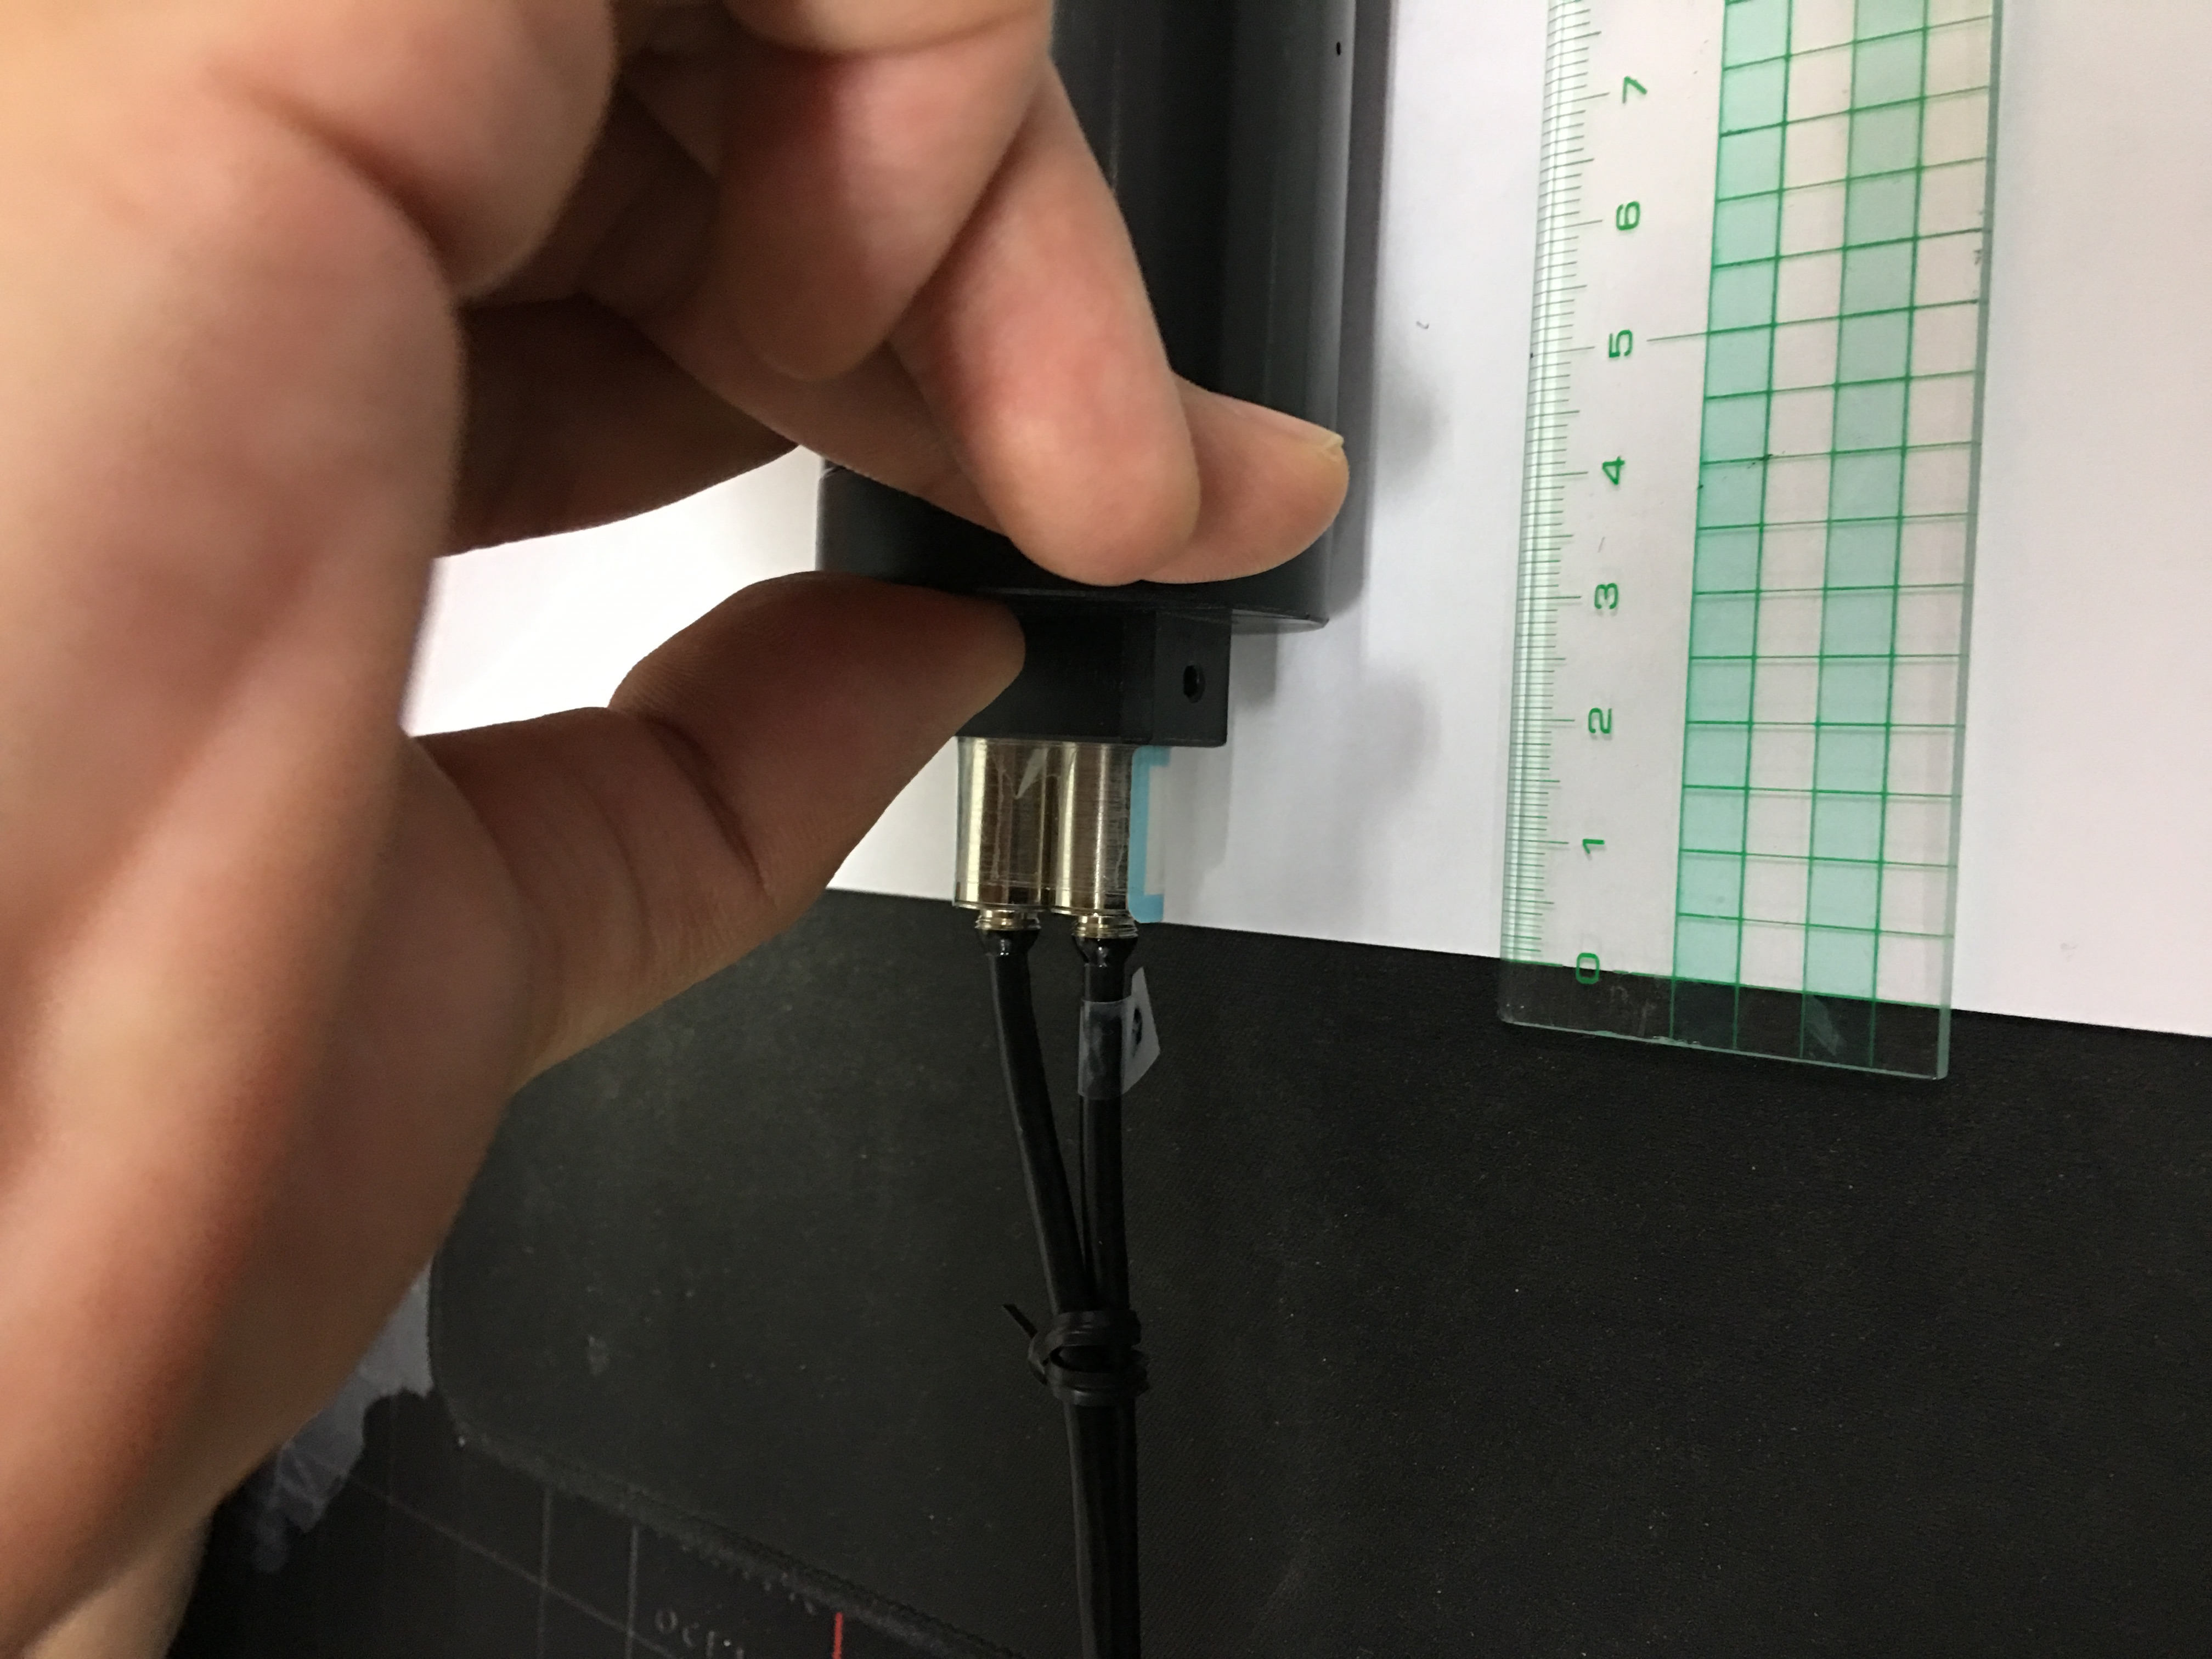
\includegraphics[width=0.6\textwidth,angle=45]{img01.jpg}
%\end{center}
%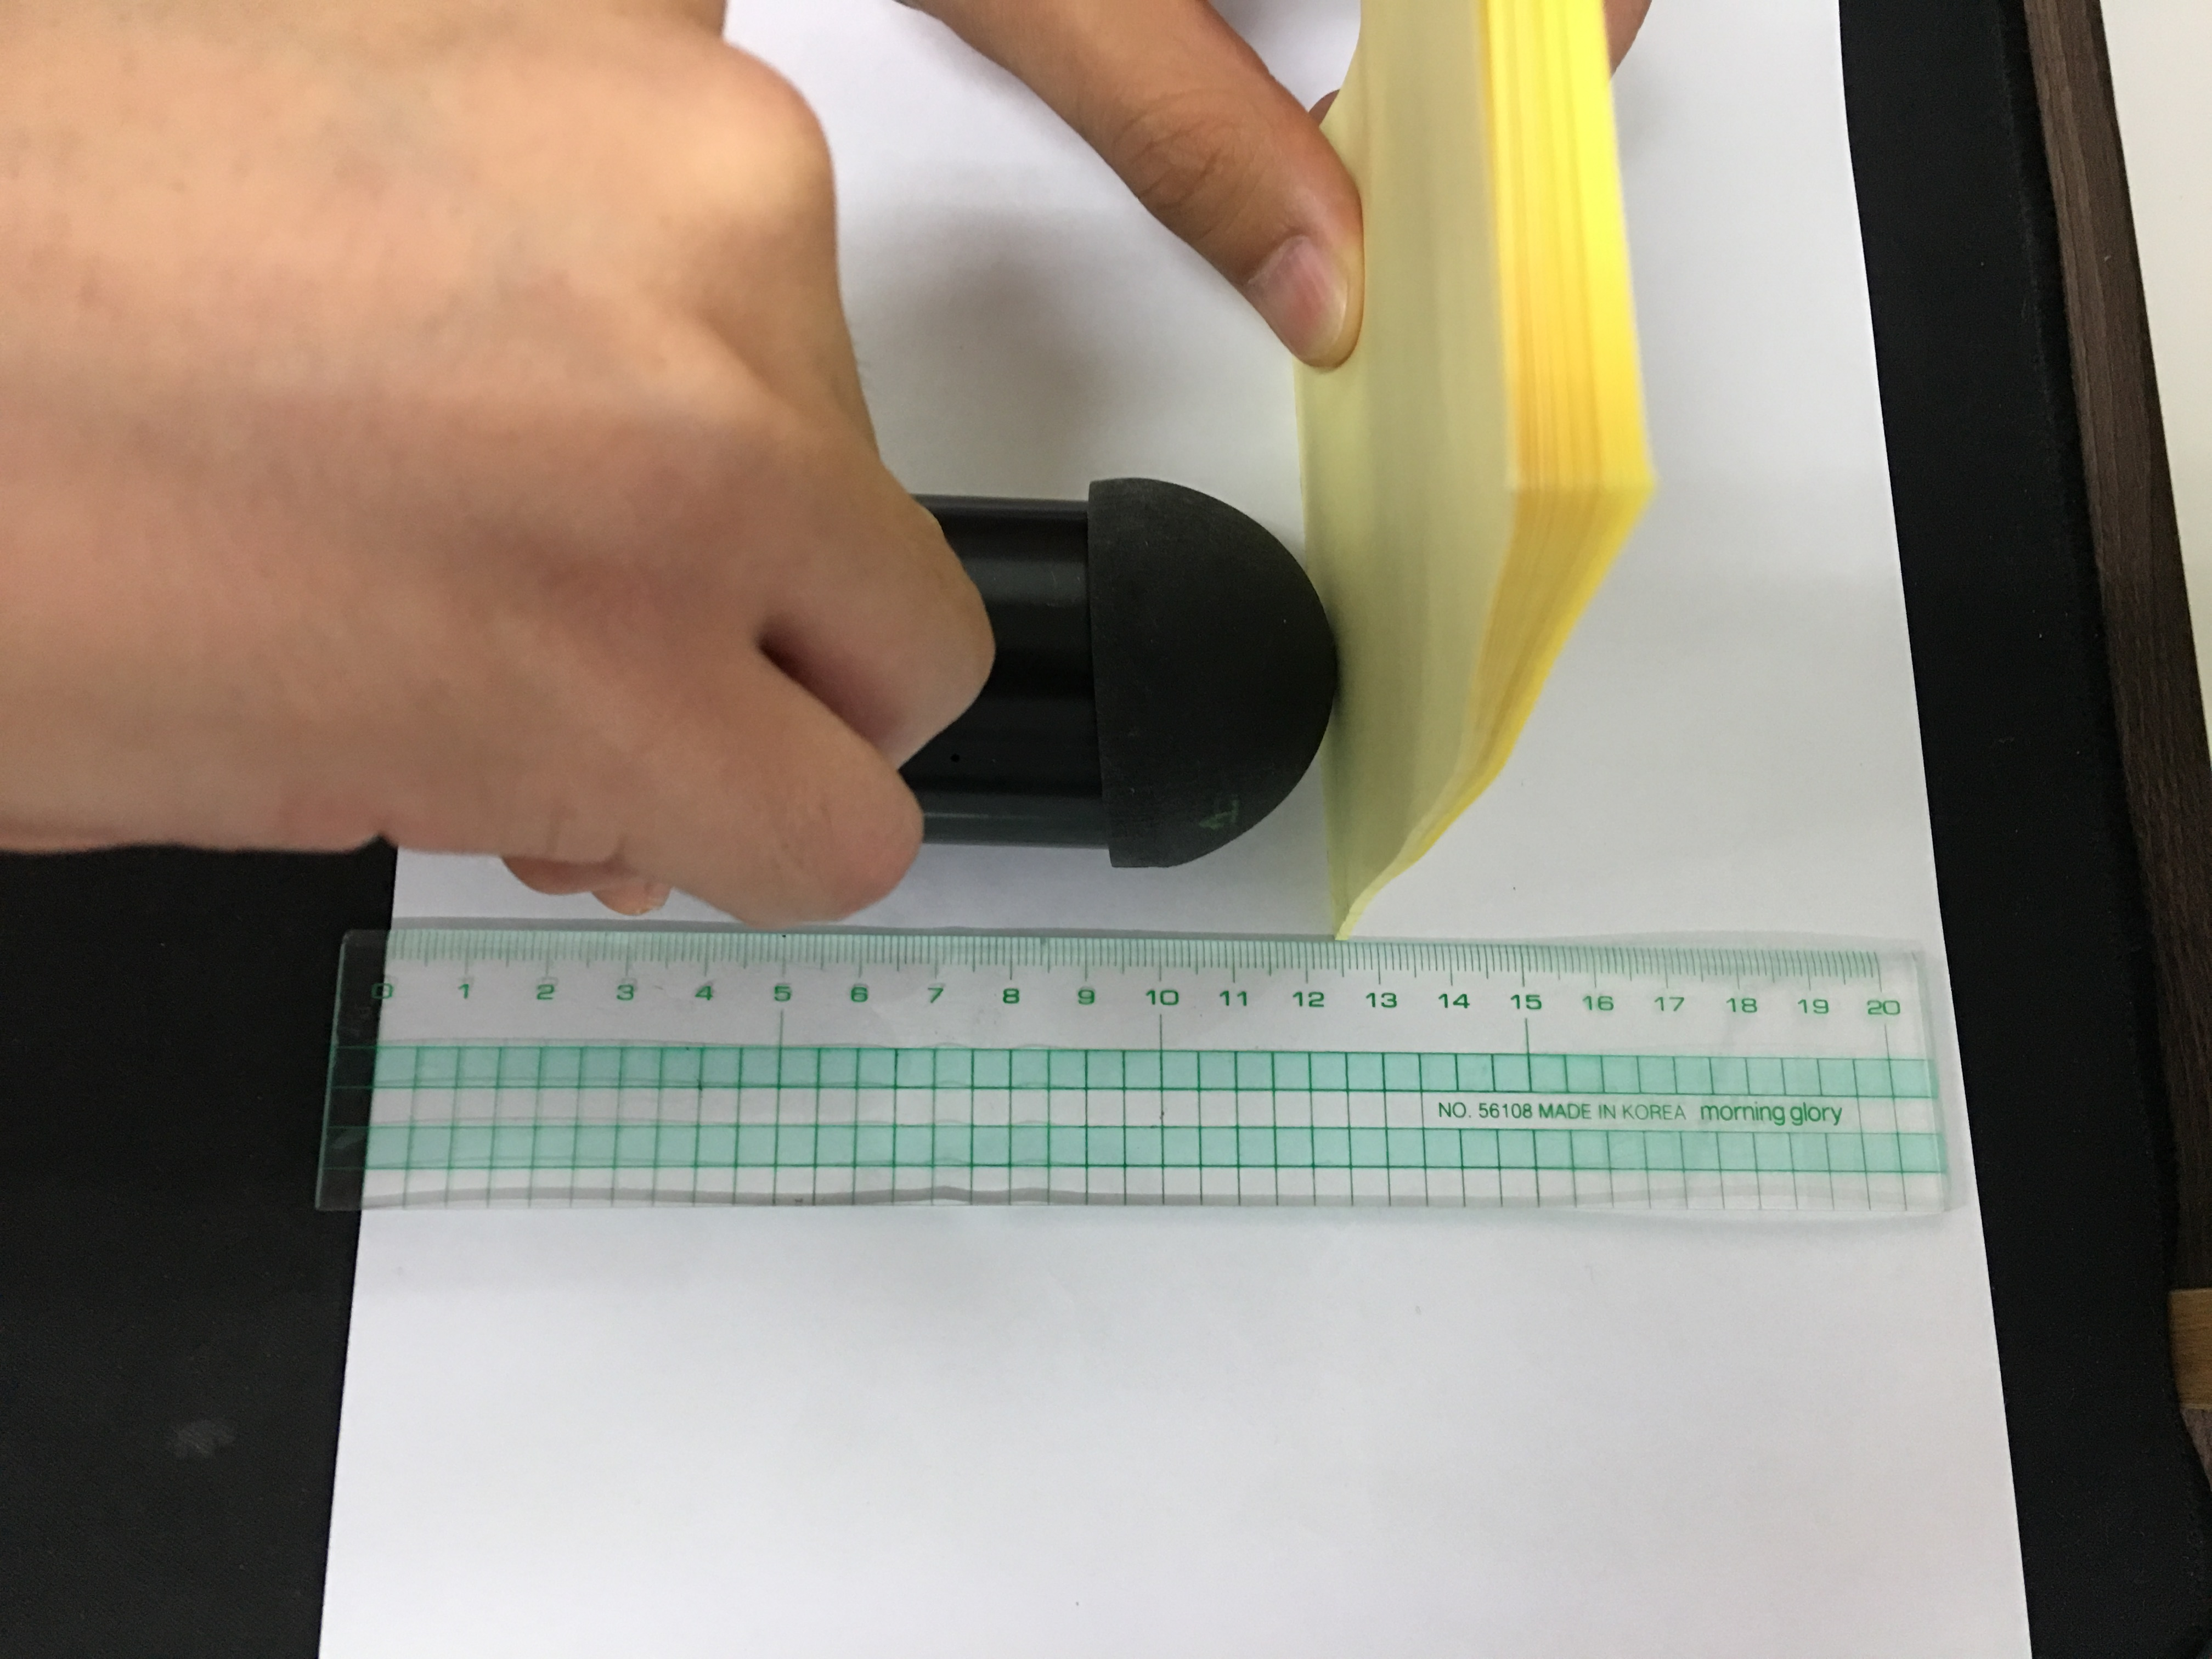
\includegraphics[height=6cm]{pictures/img02.jpg}
% \columnwidth, \textheight, \textwidth

%\begin{center}
%\includegraphics[width=0.6\textwidth, page={2}]{RedVelvet}
%\end{center}

%\begin{center}
%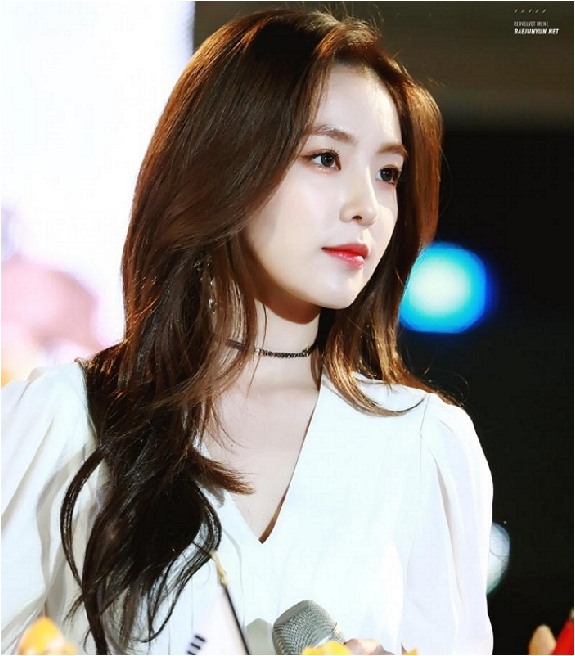
\includegraphics[width=0.6\textwidth, page={1}]{RedVelvet}
%\end{center}

%\begin{center}
%\includegraphics[width=0.6\textwidth, page={3}]{RedVelvet}
%\end{center}

%\begin{center}
%\includegraphics[width=0.6\textwidth, page={5}]{RedVelvet}
%\end{center}

\begin{figure}
\centering
\includegraphics[width=0.6\textwidth, page={4}]{RedVelvet}
\caption{가즈아!!!!} \label{fig:1}
\end{figure}

\ref{fig:1}\를 참고라하.

\begin{figure}
\centering
\quad
\subfloat[아이린]
{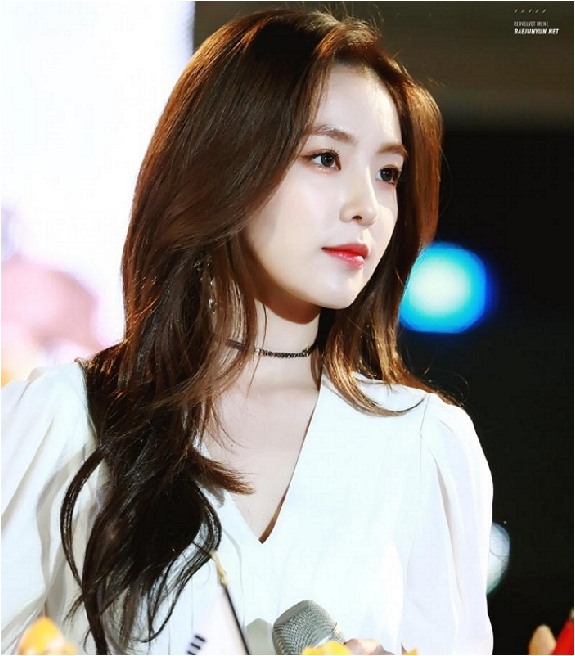
\includegraphics[page={1},height=0.2\textheight]{RedVelvet}}
\quad
\subfloat[슬기]{\includegraphics[page={3},height=0.2\textheight]{RedVelvet}}
\quad
\subfloat[조이]{\includegraphics[page={2},height=0.2\textheight]{RedVelvet}}
\quad
\subfloat[웬디]{\includegraphics[page={4},height=0.2\textheight]{RedVelvet}}
\quad
\subfloat[예리]{\includegraphics[page={5},height=0.2\textheight]{RedVelvet}}
\caption{레드벨벳}
\end{figure}
\jiwon[1-4]

\jiwon

\begin{figure}
\centering
\subfloat[아이린]
{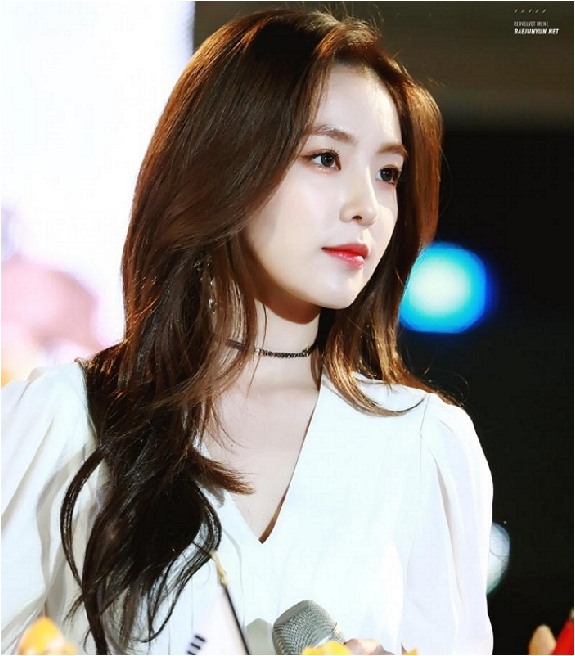
\includegraphics[page={1},height=0.2\textheight]{RedVelvet}}
\quad
\subfloat[슬기]{\includegraphics[page={3},height=0.2\textheight]{RedVelvet}}
\quad
\subfloat[조이]{\includegraphics[page={2},height=0.2\textheight]{RedVelvet}}
\caption{레드벨벳}
\end{figure}
\jiwon[1-4]

\begin{figure}
\ContinuedFloat
\centering
\subfloat[웬디]{\includegraphics[page={4},height=0.2\textheight]{RedVelvet}}
\quad
\subfloat[예리]{\includegraphics[page={5},height=0.2\textheight]{RedVelvet}}
\caption{레드벨벳}
\end{figure}
\jiwon[5-6]

\begin{tabu} to \linewidth {|X[c] | X[c] | X[c] | X[c] |}\hline
\TeX & \LaTeX & \XeTeX & \LuaTeX \\ \hline
\end{tabu}
\bigskip

\begin{tabu} to 8cm {|X[c] | X[c] | X[c] | X[c] |} \hline
\TeX & \LaTeX & \XeTeX & \LuaTeX \\ \hline
\end{tabu}
\bigskip

\begin{tabu} spread 0pt {|X[c] | X[c] | X[c] | X[c] |} \hline
\TeX & \LaTeX & \XeTeX & \LuaTeX \\ \hline
\end{tabu}
\bigskip

\begin{tabu}{X|X|X|X|X}
\hline
쌀 & 완두 & 옥수수 & 눌린보리 & 삶은고구마 \\
\hline
X & X & X & X & X \\
\hline
\end{tabu}
\bigskip

\begin{tabu}{X[2] | X[3]| X[4]}
\hline
아이쿠 나는요 & 오빠가 좋은걸 어떻개 & I'm in my dream \\
\hline
X & X & X \\
\hline
\end{tabu}
\bigskip

\begin{tabu} spread 10pt
{|X|[2pt, OliveDrab] X|[5pt, Plum] X|[10pt, RedViolet]}
탄한 녹색 & 자두색 & 붉은 빛 오렌지
\end{tabu}
\bigskip

\begin{tabu}{X X X X}
해리포터 & 레이 & 루크 & 프로도 \\ \tabucline[1pt on2pt Plum]{}
볼드모트 & 카일로 렌 & 다스 베이더 & 사우론 \\ \tabucline[1pt on2pt Blue]{2-3}
\end{tabu}
\bigskip

\begin{tabu}{X[0.7]| X[1.4]| X[1.2]| X[1]| X[1]| X[0.7]| X[0.5]} \hline
\tiny
& 더불어민주당 & 자유한국당 & 국민의당 & 바른정당 & 정의당 & 기타 \\ \hline
의석수 & & & & & & \\ \hline
\end{tabu}
\bigskip

\begin{tabu} to 0.4 \textwidth {X[c] | X[c]}
\hline
\multirow{5}{*}{레드벨벳} & 아이린 \\ \tabucline{2}
& 슬기 \\ \tabucline{2}
& 웬디 \\ \tabucline{2}
& 조이 \\ \tabucline{2}
& 예리 \\ \hline
\end{tabu}

\end{document}